% Standard template book
\documentclass[11pt, a4paper, oneside]{book}

%%%%%%%%%%%%%%%%%%%%%%%%%%%%%
% Packages
%%%%%%%%%%%%%%%%%%%%%%%%%%%%%

% Better looking urls
\usepackage[hyphens]{url}

% During testing to se all the margins
% \usepackage[showframe]{geometry}
% Package parskip is supposed to fix whitespaces in list
% and other environments when you alter the \parskip setting.
% https://en.wikibooks.org/wiki/LaTeX/Paragraph_Formatting
\usepackage{parskip}

% Remove indentation of first line in each paragraph
\setlength{\parindent}{0cm} % Default is 15pt.

% Add whitespace between paragraphs
\setlength{\parskip}{3mm plus4mm minus3mm}

% Alter headers and footers
\usepackage[pagestyles]{titlesec}
\newpagestyle{footerPageNumberMiddle}{\setfoot[\thepage][][]{}{\thepage}{}}

% Adding \figure support
\usepackage{graphicx}

% Add support for list of abbreviations
\usepackage{nomencl}
\makenomenclature
\setlength\nomlabelwidth{2cm} % Change this value to align the list of abbrev.

% Caption support in figures
% with sub-figures
\usepackage[hypcap=true]{caption}
\usepackage[hypcap=true,list=true,listformat=simple]{subcaption}

% Add links within the PDF
% All links are turned into booksmarks as well
\usepackage[bookmarks, hidelinks]{hyperref}

% Make sure hyperlinks to figures link to top of image
% and not to the caption.
\usepackage[all]{hypcap}

% Make it possible to add bookmarks without entries in the
% table of content.
\usepackage{bookmark}


%%%%%%%%%%%%%%%%%%%%%%%%%%%%%
% Document start and frontmatter
%%%%%%%%%%%%%%%%%%%%%%%%%%%%%
\begin{document}
\frontmatter

% Title
\title{Thesis title}

% Author
\author{Firstname Surname}

\maketitle

%%%%%%%%%%%%%%%%%%%%%%%%%%%%%
% Abstract
%%%%%%%%%%%%%%%%%%%%%%%%%%%%%

\cleardoublepage
\pdfbookmark{Abstract}{Abstract}
\chapter*{Abstract}
\thispagestyle{empty} % No page numbering on this page
Space Plug-and-Play Architecture (SPA) is a set of standards to make it easier
to build small satellites. Focus is put on improving the integration phase and
the time consuming validation and verification process by introducing
plug-and-play functionality. From mission call-up to operational satellite it
should only take six days.

A SPA network consists of several different types of subnets with different
pros and cons. For each processing node there must be one Local Subnet Manager
(SM-L). The SM-L can communicate over different communication protocols
depending on how the respective local subnet is set up, one option is UDP/IP.

In this thesis Ada Protected Objects is presented as a viable option for
inter-process communication instead of UDP/IP in a SPA network. This thesis
present the initial work towards a SPA Local Subnet Adaptation that builds on
language constructs in Ada such as Ada Tasks and Protected Objects.  The system
design and implementation is verified deadlock free with UPPAAL but shows
indications of livelock possibilities. The severity of these livelock
situations is discussed in the conclusion.

% Keywords
\textbf{Keywords:} Space plug-and-play Architecture, SPA, UPPAAL, Timed
automata, Ada, Ravenscar, Unified Common Architecture, UNICA, Virtual Network
Protocol, VNP


%%%%%%%%%%%%%%%%%%%%%%%%%%%%%
% Acknowledgement
%%%%%%%%%%%%%%%%%%%%%%%%%%%%%

\cleardoublepage
\pdfbookmark{Acknowledgement}{Acknowledgement}
\chapter*{Acknowledgement}
\thispagestyle{empty} % No page numbering on this page
TODO


%%%%%%%%%%%%%%%%%%%%%%%%%%%%%
% Table of Content, List of Figures/Tables
%%%%%%%%%%%%%%%%%%%%%%%%%%%%%

\cleardoublepage
\pdfbookmark{\contentsname}{Contents}
\tableofcontents

\listoffigures
\addcontentsline{toc}{chapter}{\listfigurename}
\listoftables
\addcontentsline{toc}{chapter}{\listtablename}

% List of Abbrevations
% To align the columns change the value further up in this file next
% to loading the nomencl package.
\renewcommand{\nomname}{List of Abbreviations}
\cleardoublepage%
\printnomenclature
\addcontentsline{toc}{chapter}{\nomname}

%%%%%%%%%%%%%%%%%%%%%%%%%%%%%
% Mainmatter - The Report
%%%%%%%%%%%%%%%%%%%%%%%%%%%%%

\mainmatter
\pagestyle{footerPageNumberMiddle}
\chapter{Introduction}

\section{Background}
TODO: Summary of the State of the Art.

\section{Problem Statement}
TODO: Definition of the problem statement(s).

TODO: Define the different properties/attributes to be measured when comparing
event-triggered and time-triggered systems.

TODO: Define what is in scope and what is out of scope.

\section{Structure of this report}
TODO: Add one paragraph with information on how the following chapters and
sections are structured. This section title might not be needed for this
paragraph.

\chapter{Method}\label{ch:method}
\section{Literature study}
The literature study was conducted by selecting different key terms related to
the topics and searching for them in two different search engines. The first
one was Google scholar and the second one was the "Discovery" search engine
available for Mälardalen University's students and employees. The Discovery
search engine search through multiple databases such as IEEE Xplore,
ACM Digital Library and SpringerLink. For searches in the Discovery search
engine only articles with full text available was requested.

In Google scholar the first 20 results were looked into and the first 40
results given by Discovery search engine was looked into. Only results with
full text PDFs were selected from Google Scholar.

A first read through of abstracts was conducted to filter out unrelated
papers and then followed by a read through of introductions and conclusions for
another filtering round. The key terms selected are shown below under
respective topic's section.

\subsection{Space plug-and-play Architecture}
The key terms chosen was "Space plug-and-play Avionics", "Space
plug-and-play Architecture" and "why Space plug-and-play Avionics".

All references from two relatively new reports were looked into as well.

% space plug-and-pay avionics
%AFRL plug and play spacecraft avionics.
%developing an ontology.

\subsection{Dependability and Ada}
\subsection{Model Checking and UPPAAL}
\subsection{Internet of Things}

\section{An Agile Unified Process}
\subsection{Requirements Analysis}
TODO: Write down how I did the requirements analysis and which references I
used for guidance.

\subsection{Design with UML}
TODO: Write down how I did the design and which references I used for guidance.

\subsection{Modeling, validation and verification with UPPAAL}
TODO: Write down how I did the modeling, validation and verification and which
references I used for guidance.

\subsection{Development in Ada}
TODO: Write about the development in Ada and how regression testing was done.
Test-Driven Development was used and so on.

\subsection{An iterative process}
TODO: Mention that the requirements analysis to development in Ada (sections
above) was iterated twice to improve the end result.

\chapter{Result}\label{ch:result}
\section{Model verification}
The model presented in chapter \ref{ch:designing_and_modeling} was verified
with the verification queries presented in the same chapter.

\begin{itemize}
    \item For deadlock verification the property was satisfied.
    \item For livelock verification the property was not satisfied.
\end{itemize}

% \section{Time-triggred and event-triggered systems}
% TODO: Write down the different results I found (the properties/attributes to be
% measured must be defined in the problem statement).

\section{Implementation}
The implemented SPA framework code called "Virtual Network Library" is
available on Github at \url{https://github.com/virtualnetwork/vn-lib}. The
modular design is shown in figure \ref{fig:appendix_component_overview} and the
source code compiles with the Ravenscar restrictions. Efforts has also been
made to limit the amount of dynamic memory usage.

Example implementation is available in the "examples" directory in the git
repository.

\chapter{Conclusion}\label{ch:conclusion}
Presented in this thesis report is a model-checked implementation of a new
subnet local adaptation for the Space plug-and-play Architecture, implemented
as the Virtual Network Library \cite{web:github-vn-lib} for the fork of SPA
called "Virtual Network Protocol". Instead of UDP/IP for IPC, Ada Protected
Objects are used to share data between different Ada tasks.

When model-checking a system to verify that it behaves as expected it's
important to get the model to resemble the implementation as close as possible
and the implementation to resemble the model as close possible. It's a network
of two development artifacts that prove that the system behaves according to
specifications. In this thesis the specifications are the SPA standards
and our implementation is the "Virtual Network Library" implementation with
example applications that is verified.

In chapter \ref{ch:designing_and_modeling} the process that took place to reach
the end result when it comes to UPPAAL models and implementation is shown.
Going further with an even more detailed model would go into unnecessary detail
such as how the routing tables were implemented or how the CAS table was
implemented. As the different tables are not going to hold any substancial
amount of data the time to do a lookup in the different tables are
neglectable. This leads to the conclusion that the model's level of abstraction
is about right for the goal with this thesis.

...

TODO: Is both the event- and time-triggered systems verified correcly with the
models and are the models good abstractions from the real-world implementation?
Is event- or time-triggered systems best in this field?

\section{Future research and development}
The major consequence of moving away from UDP/IP as IPC is that the
applications running on the different processing node no longer are modular in
the sense that it's easy to add and remove applications on a processing node in
a running system. When using Ada Protected Objects all applications must be
compiled together into one binary and started at the same time. This leads to
future updates must replace the entire binary and reboot the system. The
trade-off between Ada Protected Objects and a run-time modularity is something
that need to be prioritzed per project basis. For robots or satelites that are
not connected to internet the increased reliability of protected objects may be
a good trade-off. On the other side devices connected to internet that always
must be up to date security wise to protect against intrusions, the modularity
may be prioritized.  An example to this could be a refridgerator that is
connected to internet and a vulnerability is found in it's transport layer
security code. Instead of updating the entire running binary it would be enough
just to update the specific module that expose the vulnerability. Future work
should look into the possibility of keeping some run-time modularity and
introducing Ada Protected Objects.

For closed-circuit networks like remote operated vehicles and some robots,
security may not be that important but for the vast majority of devices
security need to be introduced. As soon as a device is connected to internet
and start to communicate with others it will need some kind of authentication
mechanism to allow access to its own data, it will need authorization mechanism
to be able to differentiate between different other devices regarding which
device should get access to what data. Added to this is transport encryption
(confidentiality) to prevent pervasive monitoring and the possiblitiy of
disclosing private information to active listeners (man-in-the-middle attacks).
How to add security to a SPA network with open access to internet is an
important step forward to make SPA a viable option in the world of Internet of
Things.

When starting this thesis Ada was chosen as programming language because of its
track record with software that must be dependable to high-levels. Different
ISO standards and white papers from AdaCore introduce good programming
practices, how to develop good quality software and how to use object-oriented
programming in the field of safety-critical applications. The approach all
these papers use is that the developer and/or architect need to decide upon a
few things first before starting development.

First of the project must know what kind of safety level is expected from the
system. This relates to how much testing, validation and verification must
be done in the end and throughout the development. In turn the choice of
testing, validation and verification techniques influence the choice of
programming features that can and should be used. During the development and
design in this project quite a lot of discussions went into which level of
safety that was expected, as there were no specific application in mind
there was no way to decide which techniques we were going to use to test the
system in the end. Instead time went into discussing which Ada features we
thought would be usefull and which ones we should avoid. The reasoning
behind this is that the fewer Ada constructs we use the easier it will be to
validate and verify in the future (as well as porting the system to new
architectures). Future work should take a deeper look at the different safety
standards that may be of interest and come up with firm programming guidelines
that can be used during future development.

% TODO: Routing through several subnets with different speeds. Maximum
% Transmission Unit and routing through the networks with the best throughput
% should be looked into.
%
% TODO: What should be extended with regard to VN and what could be improved with
% regard to the implementation?
% 
% TODO: To improve testing of components a IPSEC/gateway for remote location
% communication could be added. Imagine that you have a development team in USA,
% Sweden, South Africa, Japan and China. All development teams work independently
% on their own SPA components. It's the responsiblity of the team in Sweden to do
% the integration testing so instead of waiting for all others to finish their
% product and send it to Sweden (could be both hardware and software), they
% connect with a SPA IPSEC gateway to all remote locations and the remote teams
% hook up their respective component. The teams have now created a plug-and-play
% system over the internet for early integration testing. This could also be used
% for remote validation and verification, the verifier connect to a remote site
% which have the component to be verified and can thereby test remotely.
% 
% TODO: "The Implementation of a Plug-and-play Satellite Bus" writes about a
% "Mission Spacecraft Design Tool" for rapid prototyping. This sounds like a
% really cool idea. Blender or Inkscape GUI, with satellite/unmanned vehicles/IoT
% purpose. The tool could create the models used for verification and the source
% code that runs on the different processing nodes.

% \section{All references}
% TODO: Remove this section from your own report when it's done so only the
% references you use are actually added to the bibliography \cite{*}.


%%%%%%%%%%%%%%%%%%%%%%%%%%%%%
% Appendix
%%%%%%%%%%%%%%%%%%%%%%%%%%%%%

\bibliographystyle{plain}
\bibliography{../references}  % references.bib is the file with all references. 
\addcontentsline{toc}{chapter}{\bibname}

\appendix
\chapter{LaTeX examples}

\section{Example of abbrevations}
This is a short example of abbreviations are added to the list of abbrevations.
The term Fig.\nomenclature{Fig.}{Figure} is now in the List of abbrevations.
The term Img.\nomenclature{Img.}{Image} is now in the List of abbrevations.
The term Tab.\nomenclature{Tab.}{Table} is now in the List of abbrevations.
The term Long Name.\nomenclature{Long Name Long Name}{This is an example of a long
abbrevation that has an even longer description that will hopefully span at
least two rows.} is now in the List of abbrevations.


\section{Figures and images}
Lorem ipsum dolor sit amet, consectetur adipiscing elit. Sed nec ligula vel
ante placerat dapibus. Vestibulum non sollicitudin tellus. Sed varius
vestibulum libero, in euismod purus dapibus sed. Pellentesque malesuada, urna
nec lobortis egestas, felis elit varius ante, in tincidunt nunc metus id diam.
Morbi sagittis velit at ipsum sodales, in tempor nulla volutpat. Integer a
neque eros. In ipsum erat, pellentesque at dapibus eget, pretium sed risus.
Vivamus quis metus vitae felis tempus vulputate eget id lacus. Aenean sit amet
gravida quam, et ornare erat. Praesent ullamcorper mattis dolor, non interdum
orci aliquam a. In tincidunt semper lectus. Duis quis mi ac felis vehicula
mollis. Fusce molestie arcu urna, a tempor turpis mattis nec. Aenean in massa a
risus euismod aliquet vel non libero.

\subsection{One figure}

\begin{figure}[h]
    \centering
    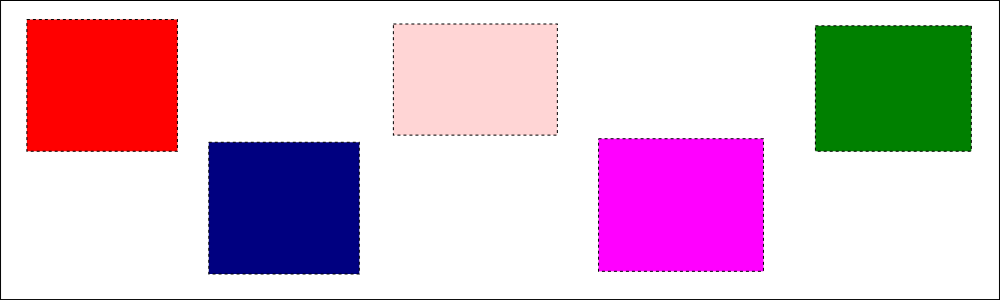
\includegraphics[width=\textwidth]{figures/test_image}
    \caption{Test Image}
    \label{fig:test_image}
\end{figure}

Aenean luctus quam ut neque viverra, quis vulputate mi hendrerit. Nunc id leo
id dui semper blandit. Nulla orci ligula, posuere non lacinia non, aliquet non
massa. Quisque gravida in mi eget volutpat. Fusce convallis felis sed dolor
ornare rhoncus. Nullam sed lacus id lectus venenatis pulvinar eget ac arcu. Sed
id turpis in leo sollicitudin euismod nec ac enim. Nunc vitae lacus lectus.
Class aptent taciti sociosqu ad litora torquent per conubia nostra, per
inceptos himenaeos. Figure \ref{fig:test_image}, Integer gravida, orci vitae
viverra ullamcorper, quam libero tempor est, non gravida magna eros id augue.
In lobortis et est auctor congue. Aliquam sed ante lacus. Vestibulum aliquam
elit eget elementum facilisis. Quisque eget felis eu leo pharetra pharetra.

\subsection{Two sub-figures}
Nulla at purus volutpat, accumsan arcu eget, commodo felis. Cras consequat
risus at rhoncus pellentesque. Aliquam tempor sodales purus in sodales. Sed ut
augue lobortis, mattis felis a, ultricies ante. Pellentesque ac tristique
ipsum, aliquet fermentum ipsum. Sed vel elit sed odio vestibulum semper id eget
enim. Nulla sed hendrerit tortor. Aliquam quam nisl, tempor ut nisl vel,
tristique facilisis libero. Suspendisse id rutrum ante. Duis sed luctus sapien.
Nullam sed quam justo.
\begin{figure}[h]
    \begin{subfigure}[b]{0.5\linewidth}
        \centering
            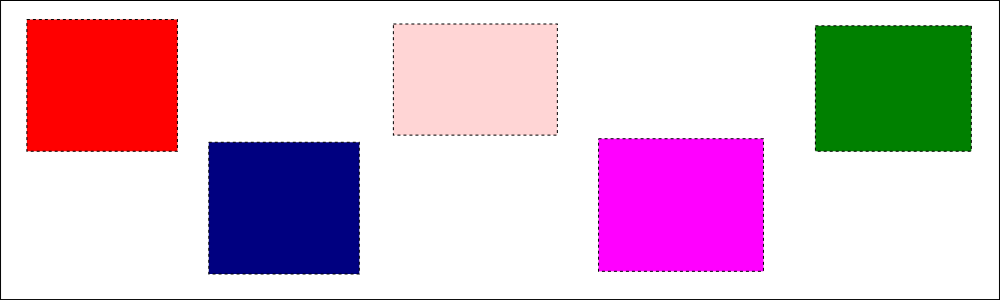
\includegraphics[width=0.9\textwidth]{figures/test_image}
            \caption{This is the caption of Sub-figure 11}
            \label{fig:subfig11}
            \end{subfigure}%
        \begin{subfigure}[b]{.5\linewidth}
            \centering
            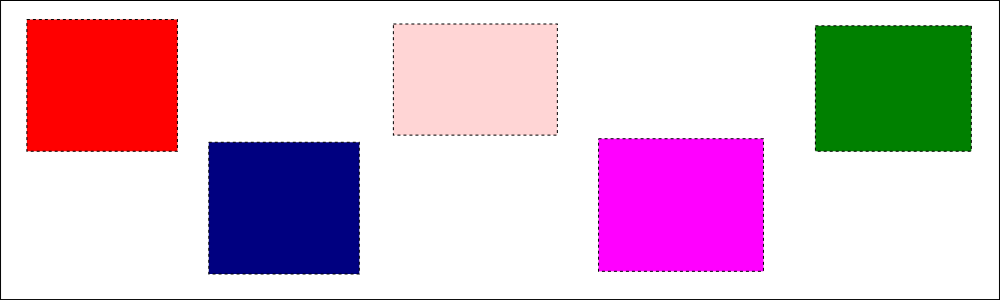
\includegraphics[width=0.9\textwidth]{figures/test_image}
            \caption{This is the caption of Sub-figure 12}
            \label{fig:subfig12}
        \end{subfigure}
    \caption{Two sub-figures}
\label{fig:sub-figures2}
\end{figure}

\subsection{Three figures together on a seperate page for floats}
Nulla at purus volutpat, accumsan arcu eget, commodo felis. Cras consequat
risus at rhoncus pellentesque. Aliquam tempor sodales purus in sodales. Sed ut
augue lobortis, mattis felis a, ultricies ante. Pellentesque ac tristique
ipsum, aliquet fermentum ipsum. Sed vel elit sed odio vestibulum semper id eget
enim. Nulla sed hendrerit tortor. Aliquam quam nisl, tempor ut nisl vel,
tristique facilisis libero. Suspendisse id rutrum ante. Duis sed luctus sapien.
Nullam sed quam justo.

\begin{figure}[p]
    \centering
    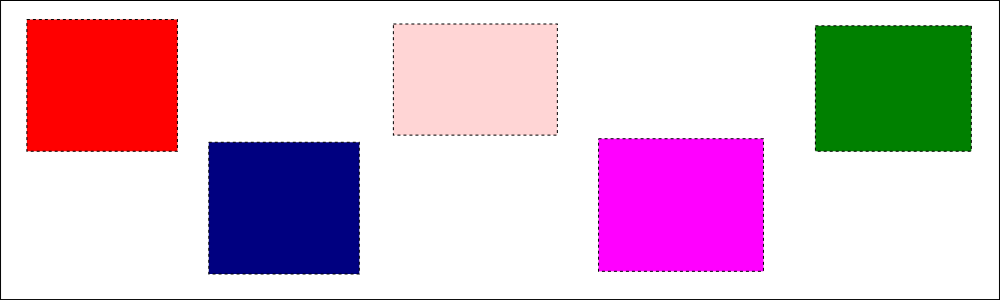
\includegraphics[width=\textwidth]{figures/test_image}
    \caption{Test Image 3}
    \label{fig:test_image3}
\end{figure}

\begin{figure}[p]
    \centering
    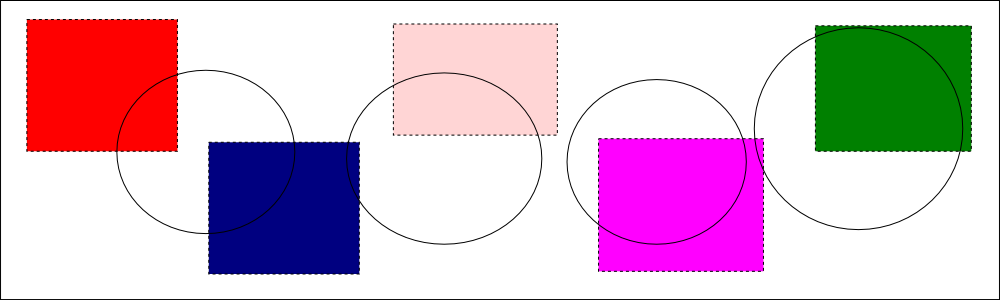
\includegraphics[width=\textwidth]{figures/test_image2}
    \caption{Test Image 4}
    \label{fig:test_image4}
\end{figure}

\begin{figure}[p]
    \centering
    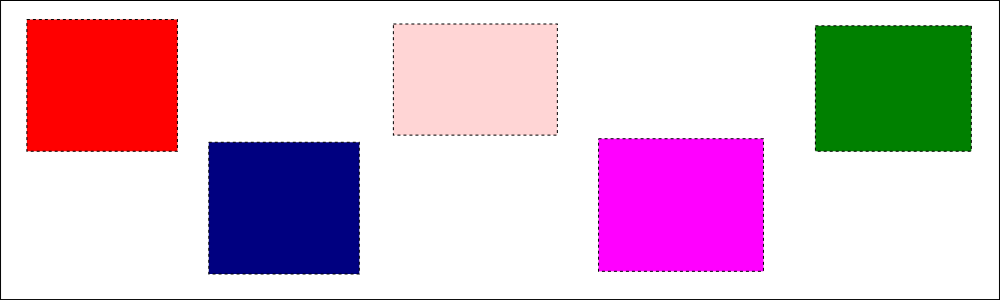
\includegraphics[width=\textwidth]{figures/test_image}
    \caption{Test Image 5}
    \label{fig:test_image5}
\end{figure}

% For more information about tables go to
% https://en.wikibooks.org/wiki/LaTeX/Tables
\section{Tables}
\subsection{One table}
Table \ref{tab:testtab2}, Aenean luctus quam ut neque viverra, quis vulputate
mi hendrerit. Nunc id leo id dui semper blandit. Nulla orci ligula, posuere non
lacinia non, aliquet non massa. Quisque gravida in mi eget volutpat. Fusce
convallis felis sed dolor ornare rhoncus. Nullam sed lacus id lectus venenatis
pulvinar eget ac arcu. Sed id turpis in leo sollicitudin euismod nec ac enim.
Nunc vitae lacus lectus.  Class aptent taciti sociosqu ad litora torquent per
conubia nostra, per inceptos himenaeos. Integer gravida, orci vitae viverra
ullamcorper, quam libero tempor est, non gravida magna eros id augue. In
lobortis et est auctor congue. Aliquam sed ante lacus. Vestibulum aliquam elit
eget elementum facilisis. Quisque eget felis eu leo pharetra pharetra.

\begin{table}[!ht]
  \centering
  \begin{tabular}{l*{6}{c}r}
      Team              & P & W & D & L & F  & A & Pts \\
      \hline
      Manchester United & 6 & 4 & 0 & 2 & 10 & 5 & 12  \\
      Celtic            & 6 & 3 & 0 & 3 &  8 & 9 &  9  \\
      Benfica           & 6 & 2 & 1 & 3 &  7 & 8 &  7  \\
      FC Copenhagen     & 6 & 2 & 1 & 3 &  5 & 8 &  7  \\
  \end{tabular}
  \caption{A floating test table.}
  \label{tab:testtab1}
\end{table}

\subsection{Two tables next to each other}
Some references to the tables on the next page, Table \ref{tab:testtab3} and
Table \ref{tab:testtab4} are sub-tables of Table \ref{tab:testtab2}. Aenean
luctus quam ut neque viverra, quis vulputate mi hendrerit. Nunc id leo id dui
semper blandit. Nulla orci ligula, posuere non lacinia non, aliquet non massa.
Quisque gravida in mi eget volutpat. Fusce convallis felis sed dolor ornare
rhoncus.

\begin{table}[!htb]
    \begin{subtable}{.5\linewidth}
      \centering
        \begin{tabular}{|r|l|}
            \hline
            7C0 & hexadecimal \\
            3700 & octal \\ \cline{2-2}
            11111000000 & binary \\
            \hline \hline
            1984 & decimal \\
            \hline
        \end{tabular}
        \caption{Caption for the first sub-table}
        \label{tab:testtab3}
    \end{subtable}%
    \begin{subtable}{.5\linewidth}
      \centering
        \begin{tabular}{|r|l|}
            \hline
            7C0 & hexadecimal \\
            3700 & octal \\ \cline{2-2}
            11111000000 & binary \\
            \hline \hline
            1984 & decimal \\
            \hline
        \end{tabular}
        \caption{Caption for the second sub-table}
        \label{tab:testtab4}
    \end{subtable}
    \caption{Caption for both tables}
    \label{tab:testtab2}
\end{table}

\subsection{One table with fixed column width}
Aenean luctus quam ut neque viverra, quis vulputate mi hendrerit. Nunc id leo
id dui semper blandit. Nulla orci ligula, posuere non lacinia non, aliquet non
massa. Quisque gravida in mi eget volutpat. Fusce convallis felis sed dolor
ornare rhoncus. Nullam sed lacus id lectus venenatis pulvinar eget ac arcu. Sed
id turpis in leo sollicitudin euismod nec ac enim. Nunc vitae lacus lectus.
Class aptent taciti sociosqu ad litora torquent per conubia nostra, per
inceptos himenaeos. Integer gravida, orci vitae viverra ullamcorper, quam
libero tempor est, non gravida magna eros id augue. In lobortis et est auctor
congue. Aliquam sed ante lacus. Vestibulum aliquam elit eget elementum
facilisis. Quisque eget felis eu leo pharetra pharetra.

\begin{table}[!ht]
  \centering
    \begin{tabular}{ | l | l | l | p{5cm} |}
    \hline
    Day & Min Temp & Max Temp & Summary \\ \hline
    Monday & 11C & 22C & A clear day with lots of sunshine.
    However, the strong breeze will bring down the temperatures. \\ \hline
    Tuesday & 9C & 19C & Cloudy with rain, across many northern regions. Clear spells
    across most of Scotland and Northern Ireland,
    but rain reaching the far northwest. \\ \hline
    Wednesday & 10C & 21C & Rain will still linger for the morning.
    Conditions will improve by early afternoon and continue
    throughout the evening. \\
    \hline
    \end{tabular}
  \caption{A floating test table with fixed column width.}
  \label{tab:testtab6}
\end{table}


\end{document}
